\subsection{k-means Clustering}

\qquad k-means clustering is a method of vector quantization, originally from
signal processing, that is popular for cluster analysis in data
mining. k-means clustering aims to partition n observations into k
clusters in which each observation belongs to the cluster with the
nearest mean, serving as a prototype of the cluster. This results in a
partitioning of the data space into Voronoi cells. \\

\begin{figure*}
  \begin{minipage}[t]{0.33\textwidth}
    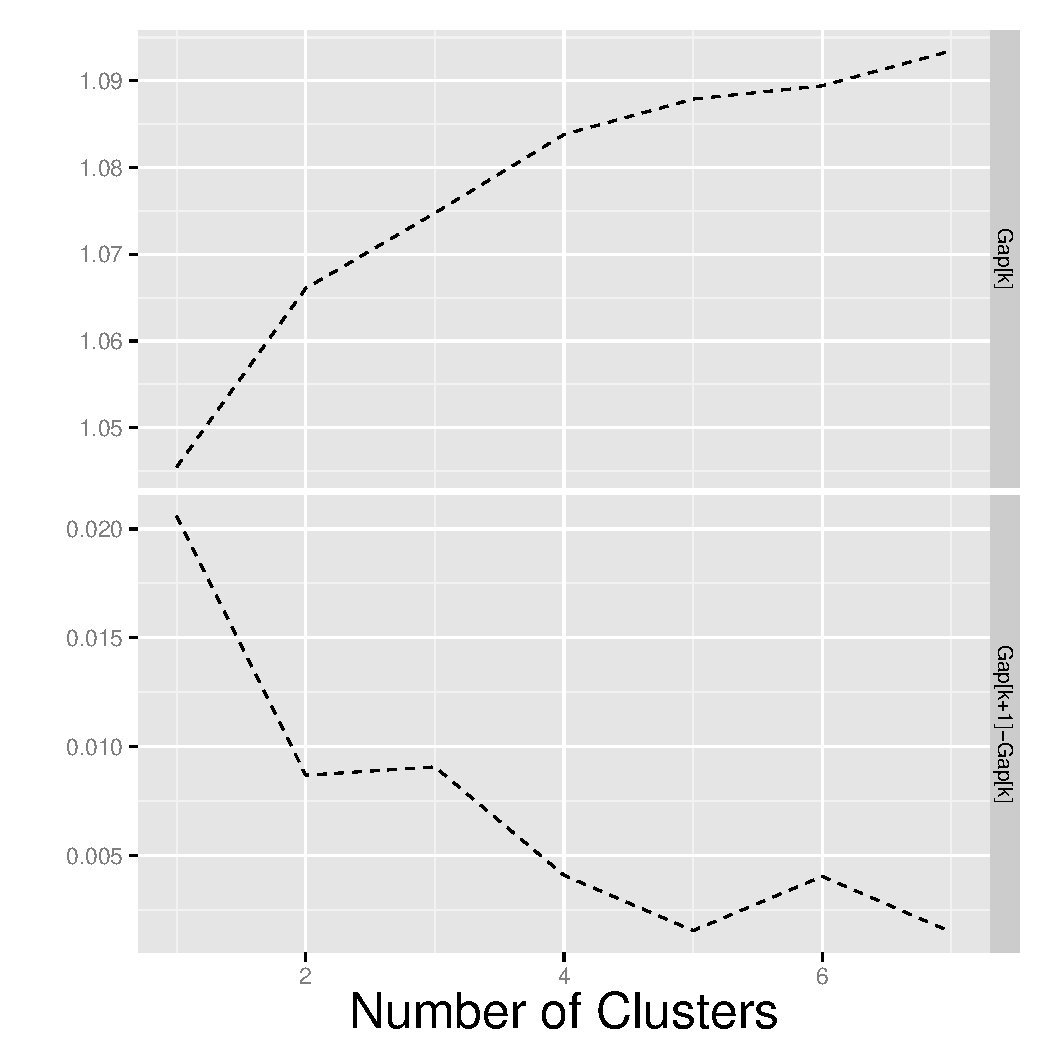
\includegraphics[width=\textwidth, height =0.8\textwidth]{fig/Gap_plot.pdf}
    \subcaption{}
  \end{minipage}
  \begin{minipage}[t]{0.33\textwidth}
    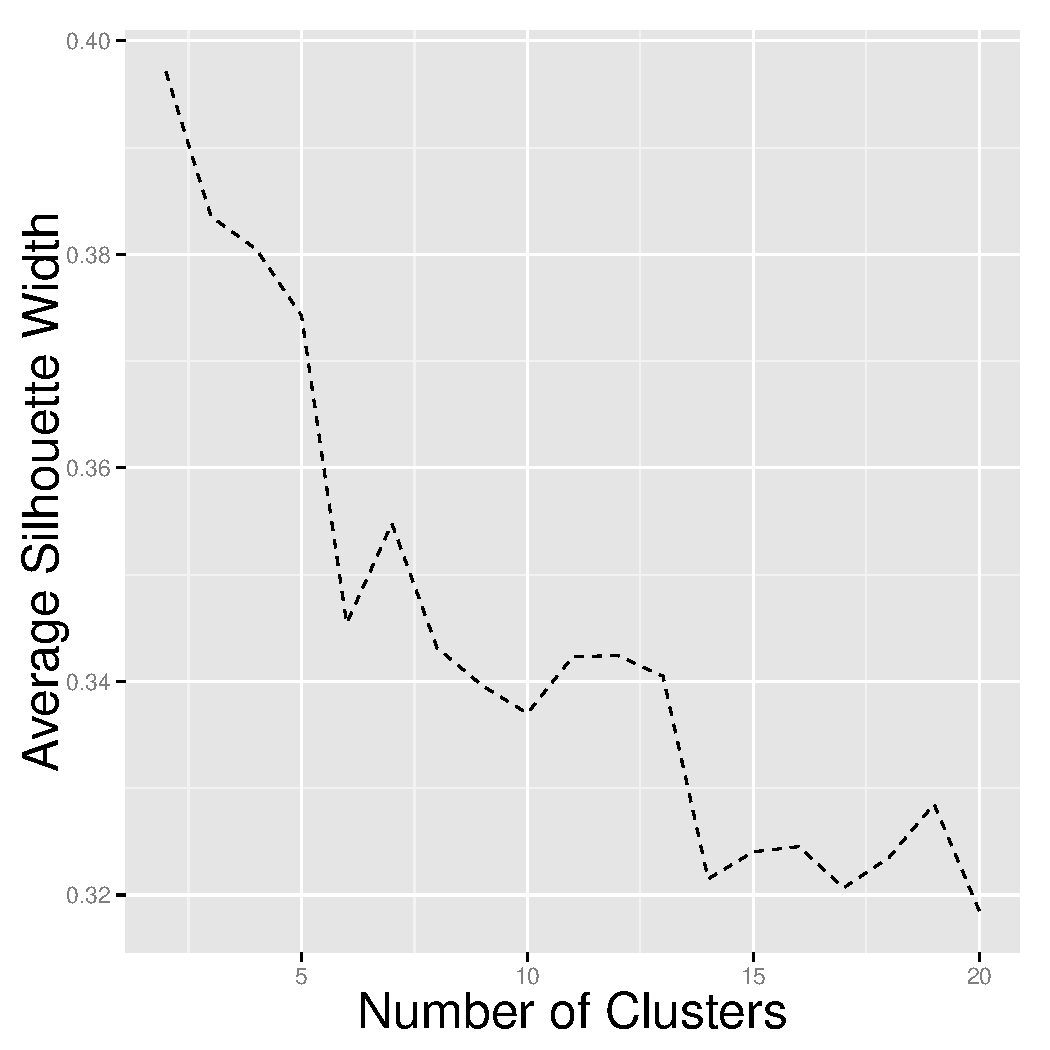
\includegraphics[width=\textwidth, height =0.8\textwidth]{fig/ave_sil.pdf}
    \subcaption{}
  \end{minipage}
  \begin{minipage}[t]{0.34\textwidth}
    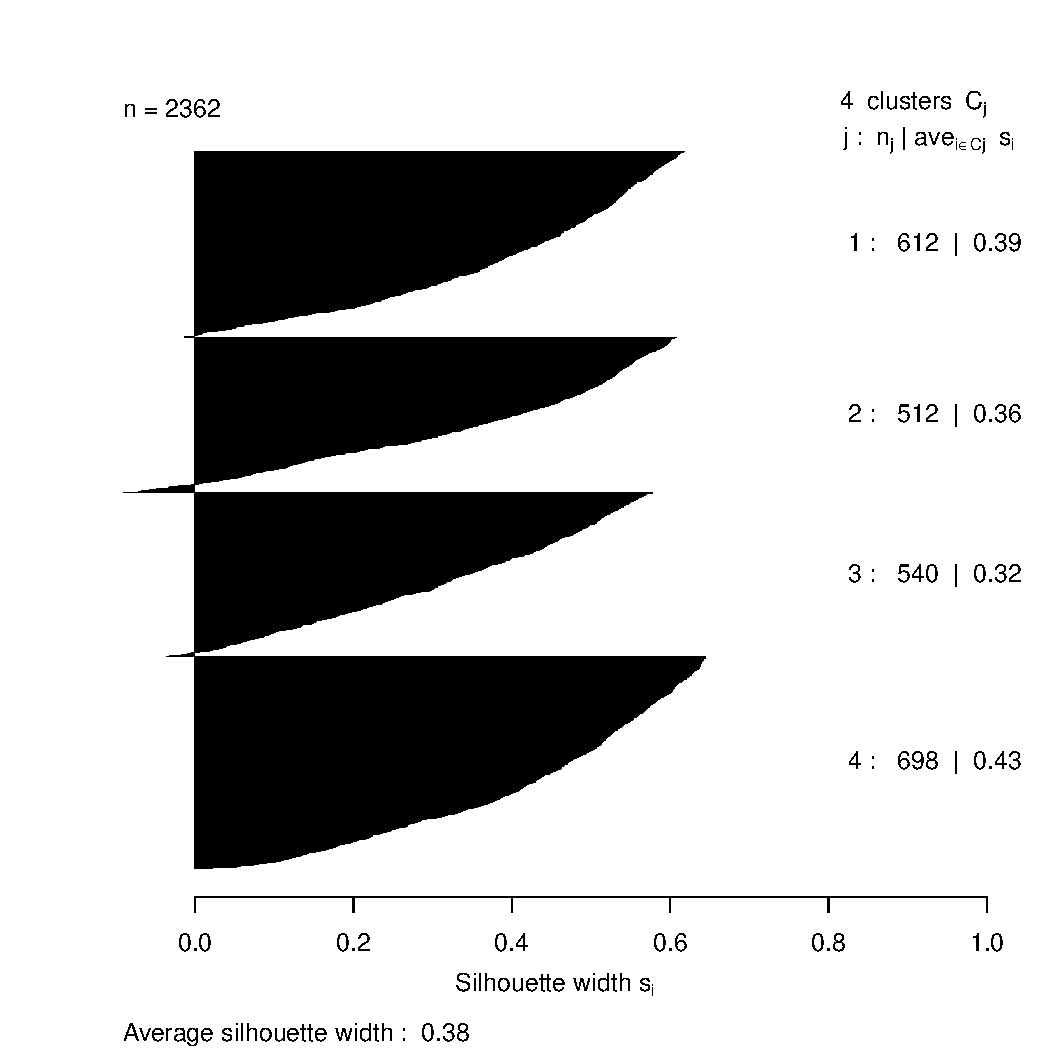
\includegraphics[width=1\textwidth, height =0.8\textwidth]{fig/sil_PCA_4.pdf}
    \subcaption{}
  \end{minipage}
  \caption{\textbf{Gap statistics and Silhouette plot for the number of clusters.} \textbf{(a)}Top: Gap statistics $Gap_k$; Bottom: The difference between consecutive Gap statistics $Gap_{k+1}-Gap_{k}$. \textbf{b} Average Silhouette width in terms of different numbers of clusters. \textbf{(c)} Silhouette plot when the number of clusters is 4.}
  \label{fig:Gap and Sil}
\end{figure*}


\qquad How to determine the number of clusters is the first concern before researches apply any kinds of clustering methods on their data. In our case, we solve the problem from both the qualitative and quantitative perspectives. The \textit{Gap} statistics \textbf([ref!]) \cite{gap} receives high popularity when it comes to \textit{k-means}. We calculate \textit{Gap} statistics for the number of clusters from 1 to 8 (See \textbf{Figure \ref{fig:Gap and Sil}(a)}). Instead of using the standard deviation of the simulated \textit{Gap} values because they are always lower than the corresponding difference, we determine to set the cutoff as 0.005. When the number of clusters goes to 4, the Gap statistics difference first falls below 0.005, hence we prefer to select 4 clusters. Furthermore, We take a look at the \textit{Silhouettes} plot \cite{silhouettes} of clustering with different numbers of clusters (See \textbf{Figure \ref{fig:Gap and Sil}(b)}). The average \textit{Silhouette} width for the number of clusters equal to 2, 3 and 4 all look good. However, combined with their associated \textit{Gap} statistics, the first two values are not preferred. Finally, the visualization also plays an important role in determining the cluster number. The rule is to find the number so that there are apparent geography groups while adding one cluster will lead to chaotic clustering (chaotic clustering means some groups distribute all over the country without obvious patterns) caused by overfitting. We compare the clustering maps with different numbers of clusters and find the map with four-clusters looks the most reasonable.\\


\qquad With slecting the cluster number as four, we apply k-means clustering on original data aggregated over county, as shown in
Figure~\ref{subfig:kmeansOnRawData}. In order to see the effectiveness 
of our data reduction, we apply k-means clustering on part of those
 principle components, i.e. the first 80, as shown in
Figure~\ref{subfig:kmeansOnReducedData}. As we can see from Figure~\ref{subfig:kmeansOnReducedData},
even only using the first 80 pcs, we can still produce a very good
cluster results, even a little bit smoother than raw data (since PCA can do denoising).\\

\qquad From the clustering results (Figure~\ref{subfig:kmeansOnRawData}), we can see \textit{New England} and \textit{Florida} belong to the red 
cluster. Many of the Northern dialects can trace their roots to this dialect which was spread westward by the New England 
settlers as they migrated west. It carries a high prestige due to Boston's early economic and cultural importance and the presence of Harvard University. 
In South Florida, there are those who consider that this region should be reclassified as part of the Northern dialect region. 
So many people from the North - particularly New York - have moved to south Florida that the majority of people tend to sound more Northern than Southern.
\textit{North Midland},
created as the people in Pennsylvania migrated westward and influenced by Scotch-Irish, German, and English Quaker settlers,  forms the central yellow cluster. The south part, is a continuous green continuum, including \textit{South Midland}, \textit{Virginia Piedmont}, 
\textit{Southern Appalachina}, and \textit{Gulf Southern}. South Midland, dominated by the Appalachian Mountains and the Ozark Mountains, was originally settled by the Pennsylvania Dutch moving south from the North Midland areas and the Scotch-Irish moving west from Virginia. In general south, as the northern dialects were originally dominated by Boston, the southern dialects were heavily influenced by Charleston, Richmond, and Savannah.
The rest of state, mainly the western regions, like \textit{Chicago Urban}, \textit{Upper Midwestern}, \textit{Rocky Mountain}, 
\textit{Pacific Northwest}, \textit{Southwestern}, and \textit{Pacific Southwest}, belong to the biggest blue continuum.
Compared with the Eastern United States, the Western regions were settled too recently for very distinctive dialects to have time to develop or to be studied in detail. Many words originally came from Spanish, cowboy jargon, and even some from the languages of the Native Americans.

\begin{figure}[t!]
    \centering
    \begin{subfigure}[t]{0.49\textwidth}
        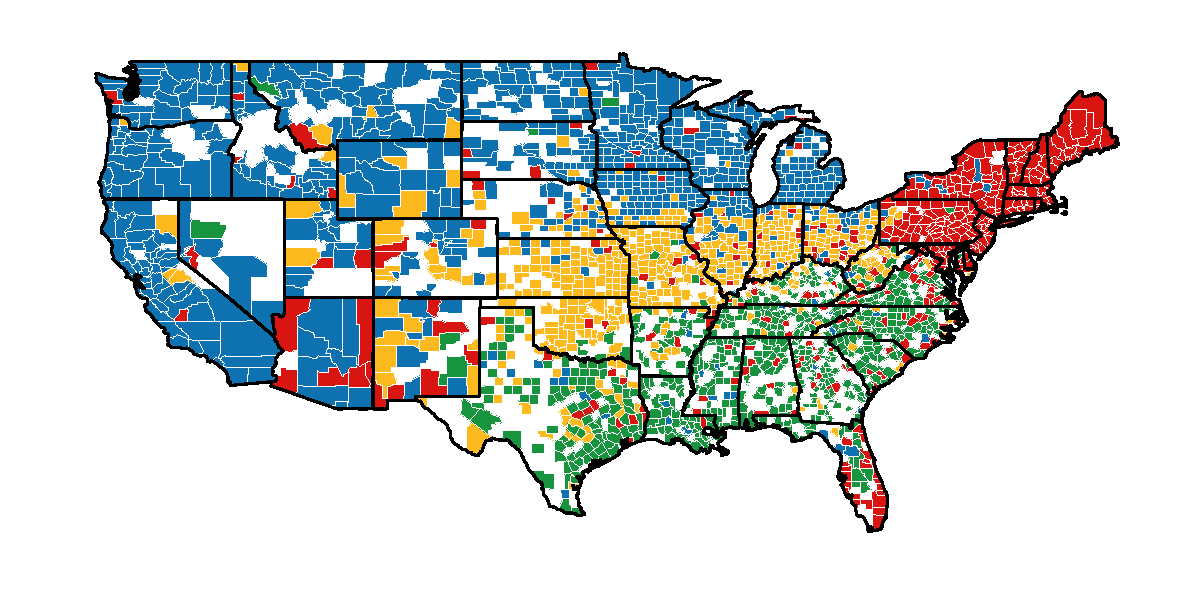
\includegraphics[width=1.1\textwidth]{fig/kmeans-original-data-4-cluster}
        \caption{raw data}\label{subfig:kmeansOnRawData}
    \end{subfigure}
    \begin{subfigure}[t]{0.49\textwidth}
        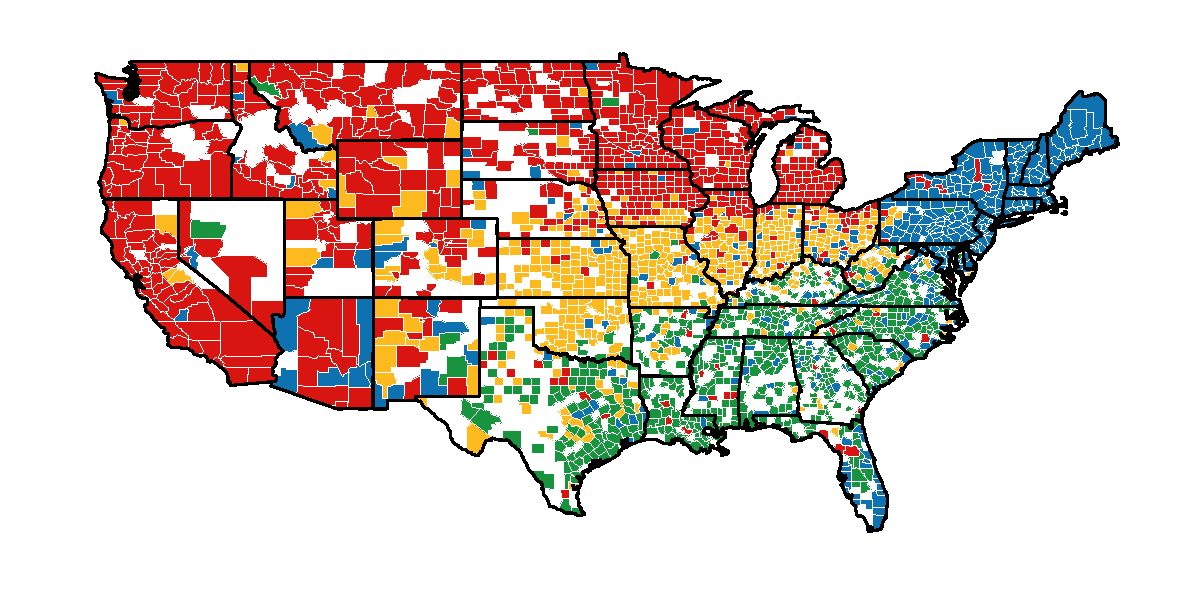
\includegraphics[width=1.1\textwidth]{fig/kmeans-reduced-data-4-cluster-80-pc}
        \caption{80 pcs}\label{subfig:kmeansOnReducedData}
    \end{subfigure}
    \caption{\textbf{The clustering map for kmeans on county level}
\textbf{(a)} raw data. \textbf{(b)} 80 pcs.}  \label{fig:kmeansClustering}
\end{figure}


\subsection{Non-negative Matrix Factorization (NMF)}

\qquad Non-negative matrix factorization, also non-negative matrix approximation is a group of 
algorithms in linear algebra where a matrix $V$ is factorized into two matrices $W$ and $H$, 
with the property that all matrices have no negative elements. NMF find applications in 
some fields as computer vision, document clustering, etc. NFM has the following form:

$$V = WH$$

\qquad It can be implemented as computing the columns vectors of $V$ as linear combination 
of the column vector of $W$ using coefficients supplied by columns of $H$.
In our case, matrix $V$ is the transpose of the original data matrix, in which each column
represents one data point (county level or person level). As NMF needs massive calculation, 
it is not realistic to do NMF on people level. Therefore, we apply NMF on the dataset 
aggregated by county.  We have done data reduction on the original dataset, i.e. PCA. 
However, here we are not able to apply NMF on reduced dataset, because NMF requires 
non-negative matrix.\\

\qquad One should realize that the results of NMF is not directly cluster ID. Instead, the 
results are coefficients of original data on the selected out ``bases''. In order to decide the 
cluster ID for each data point, here we simply choose the index of the maximal coefficient.\\

\qquad We tries $rank=3$ and $rank=4$ for NMF clustering, as shown
in Figure~\ref{fig:NMFClustering}. Comparing these plots, one can tell $rank=3$  is enough, 
because adding one more rank only bring us noises. 

\qquad It is worthy noting that, the results of NMF are essentially different from that of k-means. First, \textit{California}, \textit{Southwest} are now bunched with \textit{New England} and \textit{Florida} in the yellow cluster. This is also explainable. California actually combines elements of Western New England and Upper Midwestern. Especially, San Francisco continued to be settled by people from the Northeast and Northern Midwest, and elements of their dialects (North Midland, Upper Midwestern, Inland Northern) can be found. Mission dialect, spoken by Irish Catholics in a specific part of the city is very much like the New York City dialect. Second, \textit{Michigan} now is also in the same cluster with \textit{New England}, since the \textit{Upper Midwestern} is originally settled by people from New England and New York State who brought those dialects. Third, no matter we choose $rank=3$ or $rank=4$, the \textit{North Midland} and \textit{Upperwest} are no longer separable as in the results of k-means clustering, which is not quite explainable from a linguistic perspective. 



\begin{figure}[t!]
    \centering
    \begin{subfigure}[t]{0.49\textwidth}
        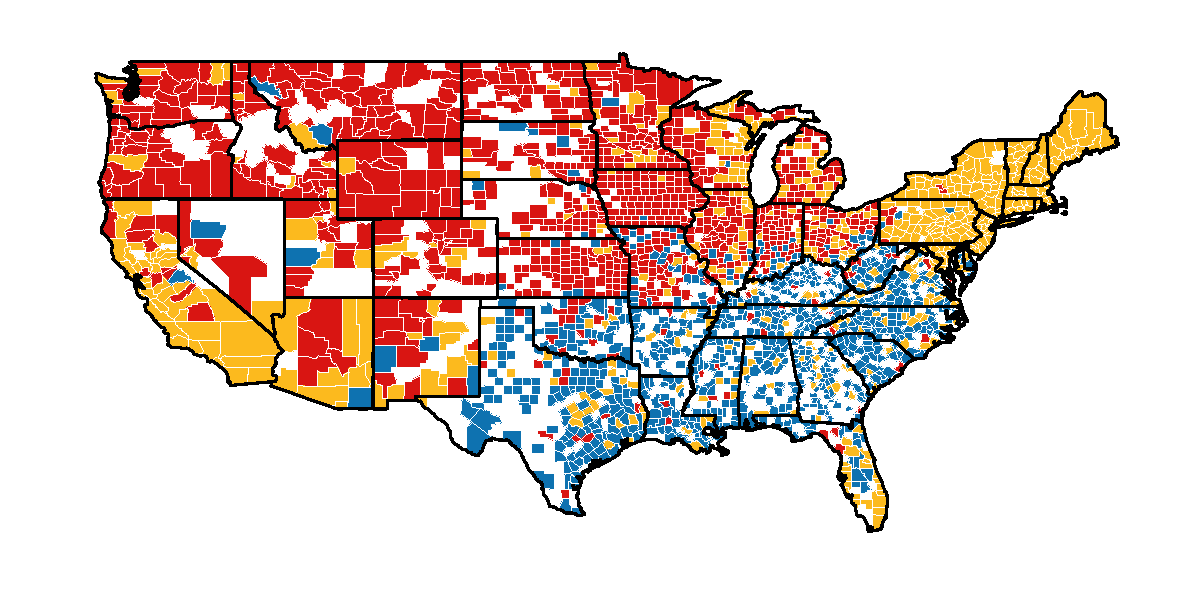
\includegraphics[width=1.1\textwidth]{fig/nmf-original-data-3cluster}
        \caption{3 clusters}\label{subfig:NMFClustering3Clusters}
    \end{subfigure}
    \begin{subfigure}[t]{0.49\textwidth}
        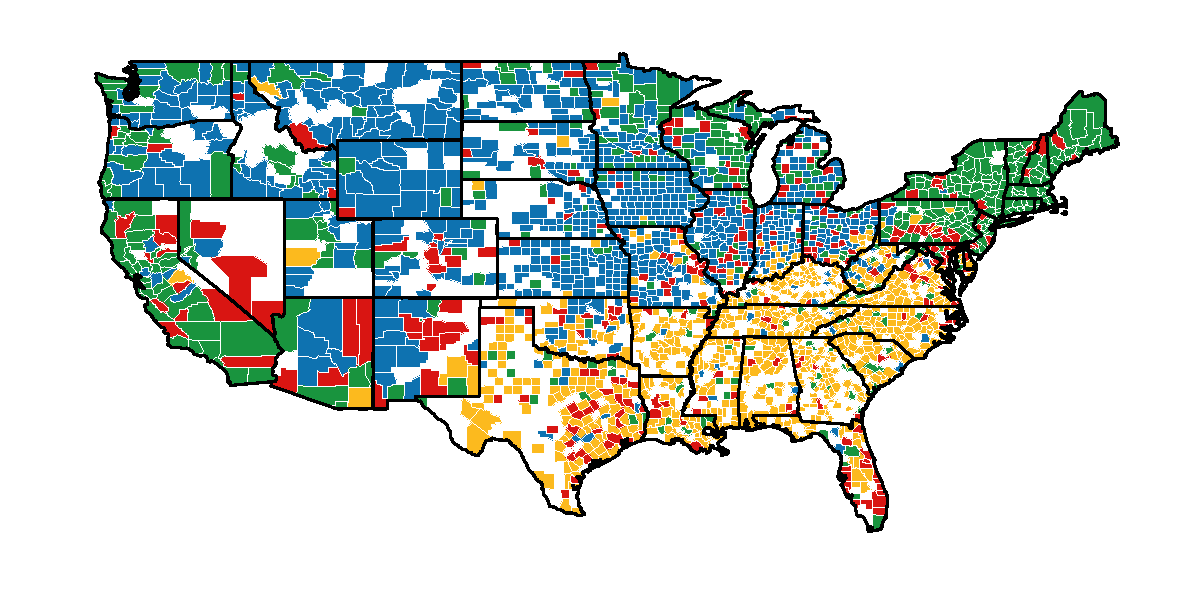
\includegraphics[width=1.1\textwidth]{fig/nmf-original-data-4cluster}
        \caption{4 clusters}\label{subfig:NMFClustering4Clusters}
    \end{subfigure}
    \caption{\textbf{The clustering map for NMF on county level}
\textbf{(a)} $k=3$. \textbf{(b)} $k=4$.}  \label{fig:NMFClustering}
\end{figure}